\documentclass{beamer}
\usetheme{metropolis}
\usepackage{graphicx}
\usepackage{amsmath}
\usepackage{tcolorbox}
\title{Elementary Statistics: Math 080}
\author{Jordan Hanson}
\institute{Whittier College Department of Physics and Astronomy}

\begin{document}
\maketitle

\begin{frame}{Course Introduction}
\begin{enumerate}
\item \textit{\textbf{\alert{What is statistical analysis?}}}
\item Math 080: Elementary Statistics
\item Read the syllabus for a roadmap
\item This is an online summer course that meets each day.
\item \textbf{Data science project and presentation}
\item Textbook: \url{https://openstax.org/details/books/introductory-statistics}
\item Download and install Excel, or LibreOffice Calc
\end{enumerate}
\end{frame}

\begin{frame}{Lecture format, with modifications}
\begin{itemize}
\item Warm-up exercise, and solution (10-15 minutes)
\item Lecture via Whiteboard and slides (10-20 minutes)
\item Interactive questions or polls (10 minutes)
\item Laboratory activity (20 minutes)
\begin{enumerate}
\item Breakout rooms
\item Offline
\end{enumerate}
\item Asynchronous content
\begin{enumerate}
\item Homework clues
\item Example problems
\item Special topics
\end{enumerate}
\end{itemize}
\end{frame}

\begin{frame}{Unit 0 Outline}
\begin{enumerate}
\item Topics from Chapter 1: 1.1, 1.2, 1.3
\begin{itemize}
\item What is a statistic?
\item Probability examples
\item Data and sampling
\end{itemize}
\item Topics from Chapter 2: 2.1 - 2.4, 2.5 - 2.8
\begin{itemize}
\item Data visualization
\item Location of the data in numerical space
\end{itemize}
\item Topics from Chapter 3: 3.1, 3.2, 3.3
\begin{itemize}
\item Two rules of probability
\end{itemize}
\end{enumerate}
\end{frame}

\section{Topics from Chapter 1}

\begin{frame}{What is statistical analysis?}
By tradition, we begin with Mark Twain.
\begin{figure}
\centering
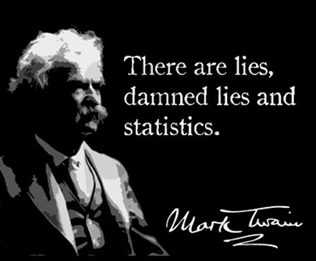
\includegraphics[width=0.6\textwidth]{figures/twain.png}
\caption{A famous quote from Mark Twain.}
\end{figure}
\end{frame}

\begin{frame}{Warm-up exercises}
\small
\textbf{COVID-19 data.}  In a March 2020 article in the magazine \texttt{wired.com}, Ferris Jabr points out that people were drawing comparisons between the influenza pandemic of 1918 and SARS-Cov-2 (COVID-19).  The \alert{case fatality rate}, or CFR, is the percentage of people who contract the disease that perish from it.  In the 1918 outbreak, it is usually stated that there were approximately 500 million infections, 50-100 million fatalities, and an overall CFR of 2.5\%.  What is interesting is that the coronavirus seems to have a CFR (averaged over age) of $\approx 3$ \%, making it ... \textit{higher}. \\ \vspace{0.5 cm}
Question 1: The above paragraph listed four pieces of data.  What are they? \\
\end{frame}

\begin{frame}{Warm-up exercises}
\small
\textbf{COVID-19 data.}  In a March 2020 article in the magazine \texttt{wired.com}, Ferris Jabr points out that people were drawing comparisons between the influenza pandemic of 1918 and SARS-Cov-2 (COVID-19).  The \alert{case fatality rate}, or CFR, is the percentage of people who contract the disease that perish from it.  In the 1918 outbreak, it is usually stated that there were approximately 500 million infections, 50-100 million fatalities, and an overall CFR of 2.5\%.  What is interesting is that the coronavirus seems to have a CFR (averaged over age) of $\approx 3$ \%, making it ... \textit{higher}. \\ \vspace{0.5 cm}
Question 2: Which number, if any, seems to have a problem?
\begin{itemize}
\item A: The total number of infections in 1918
\item B: The total number of deaths in 1918
\item C: The 1918 influenza CFR
\item D: The 2020 coronavirus CFR
\end{itemize}
\end{frame}

\begin{frame}{Warm-up exercises}
\small
\textbf{COVID-19 data.}  In a March 2020 article in the magazine \texttt{wired.com}, Ferris Jabr points out that people were drawing comparisons between the influenza pandemic of 1918 and SARS-Cov-2 (COVID-19).  The \alert{case fatality rate}, or CFR, is the percentage of people who contract the disease that perish from it.  In the 1918 outbreak, it is usually stated that there were approximately 500 million infections, 50-100 million fatalities, and an overall CFR of 2.5\%.  What is interesting is that the coronavirus seems to have a CFR (averaged over age) of $\approx 3$ \%, making it ... \textit{higher}. \\ \vspace{0.5 cm}
Question 3: From the rest of the data in the paragraph, estimate the proper CFR of the 1918 influenza.  Compare this number with the CFR of the 2020 coronavirus.
\end{frame}

\begin{frame}{Topics from Chapter 1}
\small
\textit{Vocabulary}:
\begin{enumerate}
\item \textbf{Probability}: The extend to which something is \textit{likely} to occur, measured by the ratio of favorable cases to the whole number of cases possible.
\item \textbf{Population}: The total collection of people, objects, or cases under investigation.
\item \textbf{Sample}: A subset of the population for which statistical data is collected.
\item \textbf{Statistic}: \textit{A statistic} is a number that represents a property of the sample.  For example: the CFR of a \textit{sample} of 2,500 coronavirus patients.
\item \textbf{Parameter}: Statistic measured from the \textit{entire} population.  A statistic attempts to reveal knowledge of a parameter.
\end{enumerate}
\end{frame}

\begin{frame}{Topics from Chapter 1}
\small
\textit{Vocabulary}:
\begin{enumerate}
\item \textbf{Representative sample}: a sample that captures all of the properties of a population. Counter-example: psychological studies using undergraduate subjects.
\item \textbf{Variable}: A property of each member of the population that can be determined, either quantitative or categorical. \textbf{Data} are the actual values.
\end{enumerate}
\end{frame}

\begin{frame}{Topics from Chapter 1}
\begin{tcolorbox}[colback=orange!10,colframe=orange!100,title=Mean: Definition 1]
Let X represent a \textit{variable} of a \textit{population}, and $x_i$ represent the actual value of the i-th member of a statistical \textit{sample} of that \textit{population}.  The arithmetic mean $\bar{x}$ of the \textit{sample} for that property is
\begin{equation}
\bar{x} = \frac{1}{N}\sum_i^{N} x_i
\end{equation}
\end{tcolorbox}
The mean of the variable X is the number $\bar{x}$ from the sample.
\end{frame}

\begin{frame}{Topics from Chapter 1}
Example 1: What's the average number of siblings in our community?
\begin{enumerate}
\item What is the population?
\item What is the sample?  (Our class).
\item What is the variable?
\item What are the data?
\end{enumerate}
\textbf{Write in the chat area the number of siblings in your family, including yourself.}
\end{frame}

\begin{frame}{Topics from Chapter 1}
Example 2: How many languages do you speak?
\begin{enumerate}
\item What is the population?
\item What is the sample?  (Our class).
\item What is the variable?
\item What are the data?
\end{enumerate}
\textbf{Write in the chat area the number of languages that you can speak.}
\end{frame}

\begin{frame}{Topics from Chapter 1}
\small
\textit{Vocabulary}:
\begin{enumerate}
\item \textbf{Proportion}: The total number of subjects in the sample that share a property, divided by the total number of subjects in the sample.
\item \textbf{Qualitative data}: Sometimes called categorical data, refers to non-numerical properties of subjects in sample (e.g. place of birth).
\item \textbf{Quantitative data}: Numerical values of variables for each subject in a sample (e.g. age).
\begin{itemize}
\item Continuous quantitative data: average hours of sleep per night
\item Discrete quantitative data: average number of siblings
\end{itemize}
\end{enumerate}
\end{frame}

\begin{frame}{Topics from Chapter 1}
Example 1: What fraction of Whittier College students live on campus?
\begin{enumerate}
\item What is the population?
\item What is the sample?  (Our class).
\item What is the variable?
\item What are the data?
\end{enumerate}
\textbf{Write in the chat area the number 1 if you live on-campus, and the number 0 if you live off-campus or with your family.} \\ \vspace{0.5cm}
Whittier College Factbook: 46.3\% of undergraduates live on-campus.
\end{frame}

\begin{frame}{Topics from Chapter 1}
Example 2: What is the proportion of students to instructors here?  (What is the student to faculty ratio of Whittier College)?
\begin{enumerate}
\item What is the population?
\item What is the sample?  (Our class).
\item What is the variable?
\item What are the data?
\end{enumerate}
\textbf{Let's sum the students here, and then there is me.} \\ \vspace{0.5cm}
Whittier College Factbook: average student to faculty ratio: 11
\end{frame}

\begin{frame}{Topics from Chapter 1}
\small
Example 3: You go to the supermarket and purchase three cans of soup:
\begin{itemize}
\item 19 ounces tomato bisque
\item 14.1 ounces lentil
\item 19 ounces Italian wedding
\end{itemize}
...and two desserts:
\begin{itemize}
\item 16 ounces pistachio ice cream
\item 32 ounces chocolate chip cookies
\end{itemize}
\textbf{Create three data sets: one quantitative discrete, one quantitative continuous, and one categorical.}
\end{frame}

\section{Interactive Questions}

\begin{frame}{Interactive Questions}
Almost always, we will give multiple-choice questions with answers A-D.  If you are lost, or need extra explanation, or just feel we are going to fast, select the letter E.  E stands for WAT...
\begin{figure}
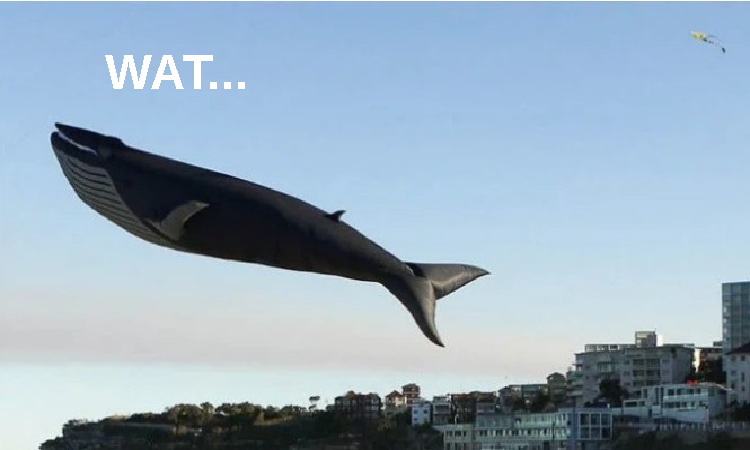
\includegraphics[width=0.5\textwidth]{figures/wat.pdf}
\end{figure}
After 1 round, we examine the \textit{answer distribution}, and if 70\% get it right, we move on.  Otherwise, we discuss via chat with each other, explaining why we picked our answer.  Then we have round 2.  Remember to hit E if you are confused.
\end{frame}

\begin{frame}{Interactive Questions}
To battle the pandemic, backup health care workers were called in to work in hospitals A, B, and C.  Hospital A began with 50, hospital B began with 40, and hospital C began with 60.  Hospital A received an additional 10, B received an additional 25, and C received an additional 5.  What is the average number of workers at hospitals in this sample (A, B, and C)?
\begin{itemize}
\item A: 53
\item B: 63
\item C: 42
\item D: 32
\end{itemize}
\end{frame}

\begin{frame}{Interactive Questions}
Suppose a sample of students record the duration of their sleep each night for a week, and gather the data at the end.  What kind of data is this?
\begin{itemize}
\item A: Quantitative discrete
\item B: Qualitative or categorical
\item C: Quantitative continuous
\item D: Variable
\end{itemize}
\end{frame}

\begin{frame}{Interactive Questions}
\begin{figure}
\centering
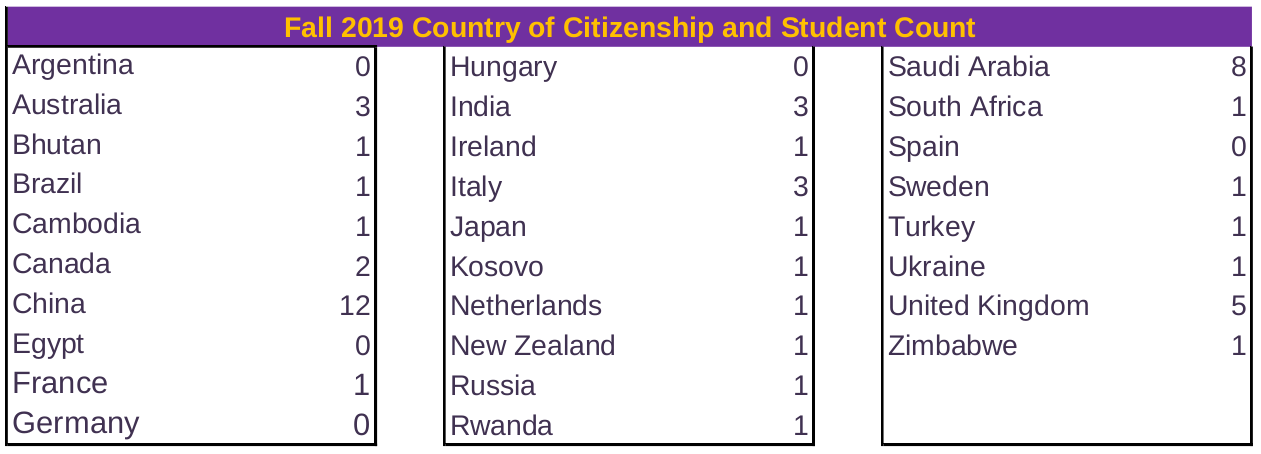
\includegraphics[width=0.85\textwidth]{figures/map.png}
\end{figure}
What kind of data is represented in the population above? (There may be more than one answer).
\begin{itemize}
\item A: Quantitative discrete
\item B: Qualitative or categorical
\item C: Quantitative continuous
\item D: Variable
\end{itemize}
\end{frame}

\begin{frame}{Interactive Questions}
\begin{figure}
\centering
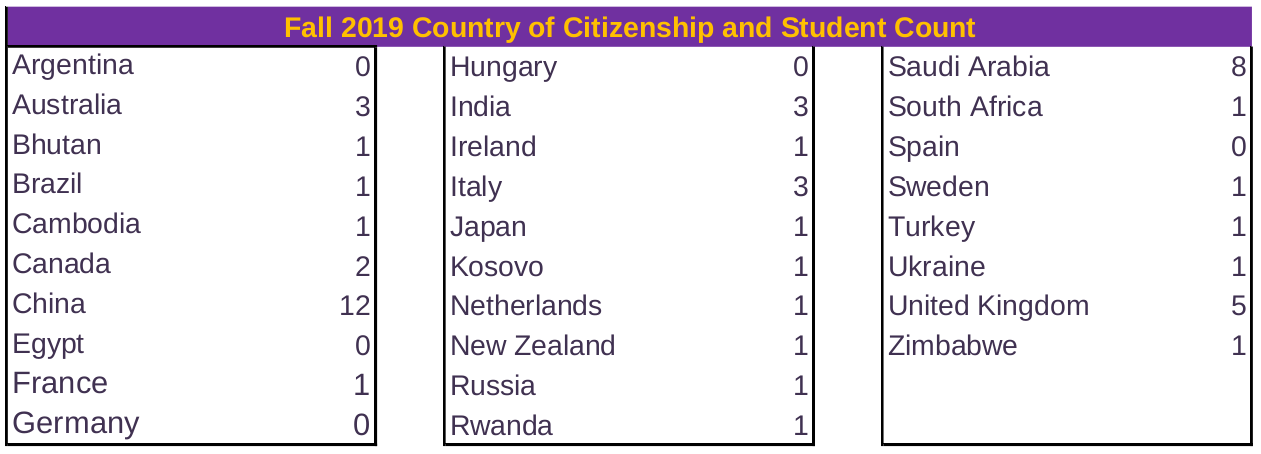
\includegraphics[width=0.85\textwidth]{figures/map.png}
\end{figure}
The total number of international students is 52 in the above table.  What proportion of international students are from China?
\begin{itemize}
\item A: 12
\item B: 12\%
\item C: 23
\item D: 23\%
\end{itemize}
\end{frame}

\begin{frame}{Interactive Questions}
\begin{figure}
\centering
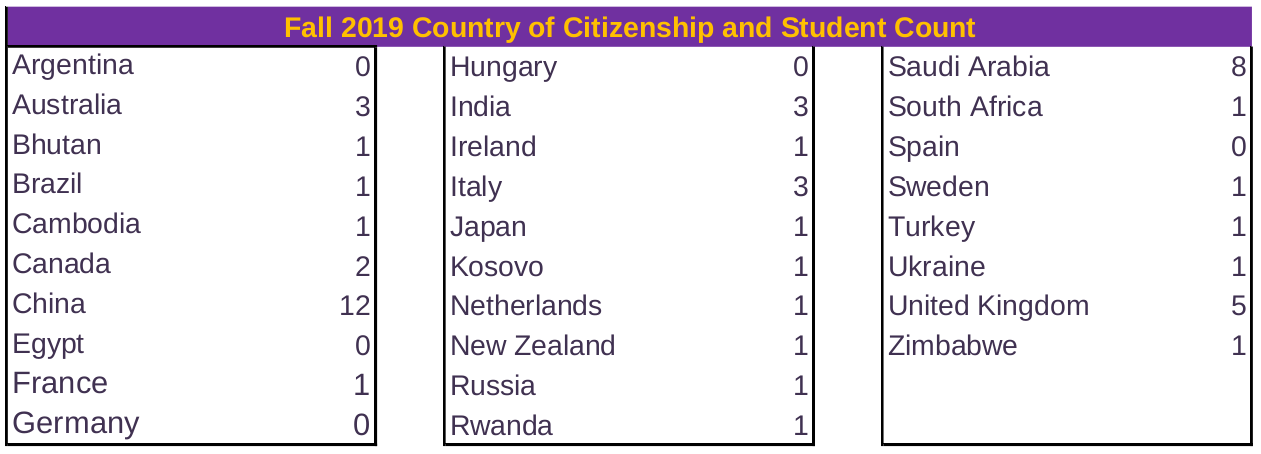
\includegraphics[width=0.85\textwidth]{figures/map.png}
\end{figure}
The total number of international students is 52 in the above table.  What proportion of international students are from Europe?
\begin{itemize}
\item A: 15\%
\item B: 23\%
\item C: 50\%
\item D: 12
\end{itemize}
\end{frame}

\section{Laboratory Activity}

\begin{frame}{Laboratory Activity}
Go to the following link and watch the interesting TED talk by Steven Levitt from 2005 about driving safety. \\ \vspace{1cm}
\url{https://www.ted.com/talks/steven_levitt_surprising_stats_about_child_carseats?utm_campaign=tedspread&utm_medium=referral&utm_source=tedcomshare} \\ \vspace{1cm}
Answer the questions on the form entitled \alert{Laboratory Exercise 1} on Moodle for this week, and submit them via email: jhanson2@whittier.edu. (This is part of your warm-ups grade...see syllabus).
\end{frame}

\section{Conclusion}

\begin{frame}{Unit 0 Outline}
\begin{enumerate}
\item Topics from Chapter 1: 1.1, 1.2, 1.3
\begin{itemize}
\item What is a statistic?
\item Probability examples
\item Data and sampling
\end{itemize}
\item Topics from Chapter 2: 2.1 - 2.4, 2.5 - 2.8
\begin{itemize}
\item Data visualization
\item Location of the data in numerical space
\end{itemize}
\item Topics from Chapter 3: 3.1, 3.2, 3.3
\begin{itemize}
\item Two rules of probability
\end{itemize}
\end{enumerate}
\end{frame}

\end{document}
